\documentclass[a4paper]{article}

\usepackage[siunitx,american]{circuitikz}
\usepackage{booktabs}
\usepackage{amsmath}
\usepackage{pgfplots}
\usetikzlibrary{intersections}

\ctikzset{bipoles/thickness=1}

\begin{document}

\paragraph{Triangle wave generator.}
\begin{center}
  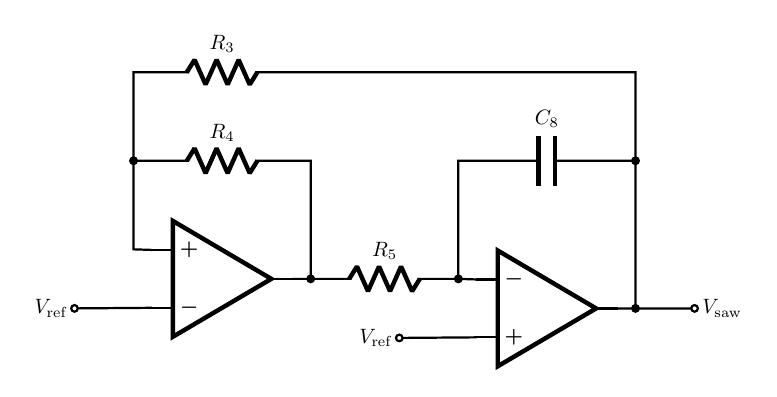
\begin{tikzpicture}[scale=0.75,transform shape]
    \draw[color=black, thick]
    (0,0) node[op amp,yscale=-1] (comp) {}
    (5.5,-0.5) node[op amp] (int) {}
    % 
    (comp.out) to (1.5,0) to [R=$R_5$,*-*] (4,0) to (int.-)
    (1.5,0) to (1.5,2) to [R,l_=$R_4$,-*] (-1.5,2) to (-1.5,0.5) to (comp.+)
    (-1.5,2) to (-1.5,3.5) to [R=$R_3$] (1.5,3.5) to (7,3.5) to (7,2)
    (4,0) to (4,2) to [C=$C_8$,-*] (7,2) to[short,-*] (7,-0.5) to (int.out)
    (7,-0.5) to[short,-o] (8,-0.5) node [anchor=west] {$V_{\text{saw}}$}
    (comp.-) to[short,-o] (-2.5,-0.5) node [anchor=east] {$V_{\text{ref}}$}
    (int.+) to[short,-o] (3,-1) node [anchor=east] {$V_{\text{ref}}$}
    ;
  \end{tikzpicture}
\end{center}
The component values are
\begin{center}
  \begin{tabular}{lS}
    \toprule
    $R_3$ & \SI{1.2}{\kilo\ohm} \\
    $R_4$ & \SI{3.0}{\kilo\ohm} \\
    $R_5$ & \SI{150}{\kilo\ohm} \\
    $C_8$ & \SI{100}{\nano\farad} \\
    \bottomrule
  \end{tabular}
\end{center}
The opamps are rail-to-rail and are powered at $V_{\text{CC}} = +\SI{5}{\volt}$. The reference voltage sits at $V_{\text{ref}} = V_{\text{CC}}/2$. The comparator switches at
\begin{equation}
  V_{\text{ref}} \pm V_{\text{th}} = \frac{1}{2} \Bigl( 1 \pm \frac{R_3}{R_4} \Bigr) V_{\text{CC}}
  =
  \SI{2.5}{\volt} \pm \SI{1.0}{\volt} .
\end{equation}
The integrator time constant is given by
\begin{equation}
  R_5 C_8 = \SI{15}{\milli\second}.
\end{equation}
The slope of the triangle wave is then given by
\begin{equation}
  \frac{V_{\text{CC}} - V_{\text{ref}}}{R_5 C_8} = \SI{166.67}{\volt/\second} .
\end{equation}
This leads to the period and frequency
\begin{equation}
  T = \Bigl( 4 \frac{R_3}{R_4} \frac{V_{\text{CC}}}{2} \Bigr) \Big/ \Bigl( \frac{V_{\text{CC}} - V_{\text{ref}}}{R_5 C_8} \Bigr) = \SI{24}{\milli\second} , \qquad
  f = 1/T = \SI{41.667}{\hertz} .
\end{equation}


\paragraph{PWM generator.}


\begin{center}
  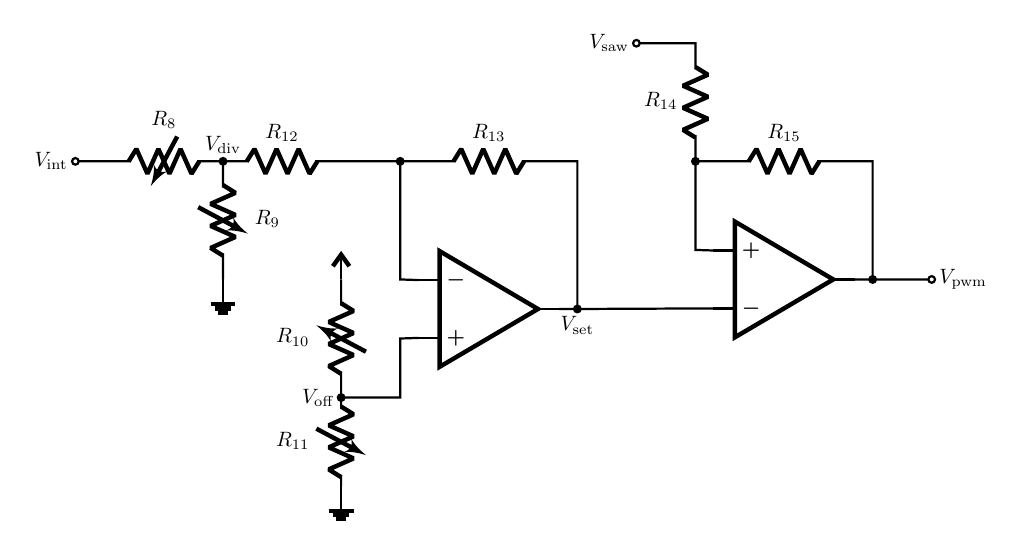
\begin{tikzpicture}[scale=0.75,transform shape]
    \draw[color=black, thick]
%
    (0,0) node [op amp] (buffer) {}
    (buffer.-) to (-1.5,+0.5) to (-1.5,+2.5) to [short,*-] (-2.5,+2.5) to[R,l_=$R_{12}$,-*] (-4.5,+2.5) to[vR,l_=$R_8$] (-6.5,+2.5) to[short,-o] (-7,+2.5) node [anchor=east] {$V_{\text{int}}$}
    (-4.5,+2.5) to[vR,l=$R_9$] (-4.5,0.5) node [ground] {}
    (-1.5,+0.5) to (-1.5,+2.5) to[R,l=$R_{13}$] (+1.5,+2.5) to [short,-*] (+1.5,0) to (buffer.out)
%
    (buffer.+) to (-1.5,-0.5) to (-1.5,-1.5) to (-2.5,-1.5) to[vR,l=$R_{10}$,*-] (-2.5,0.5) node[vcc] {}
    (-2.5,-1.5) to[vR,l_=$R_{11}$] (-2.5,-3) node[ground] {}
    %
    (5,+0.5) node [op amp,yscale=-1] (comp) {}
    (1.5,0) to (comp.-)
    (comp.+) to (3.5,+1) to (3.5,+2.5) to[R,l=$R_{15}$,*-] (6.5,+2.5) to (6.5,+0.5) to (comp.out)
    (6.5,+0.5) to [short,*-o] (7.5,+0.5) node [anchor=west] {$V_{\text{pwm}}$}
    (3.5,+2.5) to [R,l=$R_{14}$] (3.5,+4.5) to[short,-o] (2.5,+4.5) node[anchor=east] {$V_{\text{saw}}$}
%    
    (-4.5,+2.5) node [anchor=south] {$V_{\text{div}}$}
    (-2.5,-1.5) node [anchor=east] {$V_{\text{off}}$}
    (+1.5,0) node [anchor=north] {$V_{\text{set}}$}
    ;
  \end{tikzpicture}
\end{center}
\begin{center}
  \begin{tabular}{ll}
    \toprule
    $R_8$ & $\SI{30}{\kilo\ohm} + \SI{100}{\ohm} \, x$ \\
    $R_9$ & $\SI{470}{\ohm} + \SI{100}{\ohm} \, (1-x)$ \\
    $R_{10}$ & $\SI{30}{\kilo\ohm} + \SI{1}{\kilo\ohm} \, y$ \\
    $R_{11}$ & $\SI{15}{\kilo\ohm} + \SI{1}{\kilo\ohm} \, (1-y)$\\
    $R_{12}$ & \SI{150}{\kilo\ohm} \\
    $R_{13}$ & \SI{150}{\kilo\ohm} \\
    $R_{14}$ & \SI{470}{\ohm} \\
    $R_{15}$ & \SI{150}{\kilo\ohm} \\
    \bottomrule
  \end{tabular}
\end{center}
With $R_{12} = R_{13}$ the output of the first op amp sits at
\begin{equation}
  V_{\text{set}} = 2V_{\text{off}} - V_{\text{div}} , \qquad
  V_{\text{off}} = \frac{R_{11}}{R_{10} + R_{11}} V_{\text{CC}}.
\end{equation}
Since $R_{12}, R_{13} \gg R_8, R_9$
\begin{equation}
  V_{\text{div}} \approx \frac{R_9}{R_8+R_9} V_{\text{int}} .
\end{equation}
To find the desired values, we refer to the plot below.
\begin{center}
  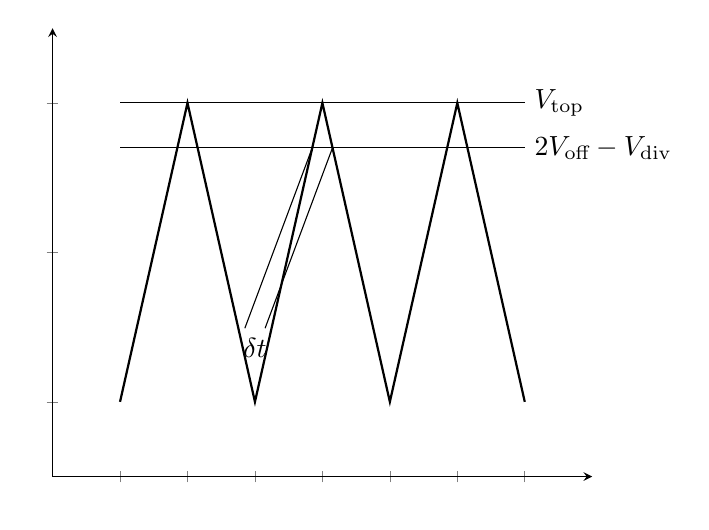
\begin{tikzpicture}
    \newcommand*{\ShowIntersection}[1]{
      \fill 
      [name intersections={of=tri and #1, name=i, total=\t}] 
      [red, opacity=1, every node/.style={above left, black, opacity=1}] 
      \foreach \s in {1,...,\t}{(i-\s) circle (2pt)
        node [above left] {\s}};
    }
    \begin{axis}[
      axis y line=left,
      axis x line=bottom,
      ymin=1,
      ymax=4,
      xmin=-12,
      xmax=84,
      xtick={0,12,...,72},
      xticklabels=\empty,
      ytick={1.5,2.5,3.5},
      yticklabels=\empty,
      clip=false
      ]

      \addplot[thick,name path global=tri] table {
        t V
        0 1.5
        12 3.5
        24 1.5
        36 3.5
        48 1.5
        60 3.5
        72 1.5
        % 84 3.5
        % 96 1.5
      };

      \addplot[name path global=top] table {
        t V
        0 3.5
        72 3.5
      };

      \addplot[name path global=set] table {
        t V
        0 3.2
        72 3.2
      };

      \path [name intersections={of=tri and set, name=i}] (i-3) coordinate (set-1) (i-4) coordinate (set-2);

      \draw (set-1) -- ($(set-1)-(0,4.19cm)$);
      \draw (set-2) -- ($(set-2)-(0,4.19cm)$);

      \node at ($(set-1)!0.5!(set-2)-(0,4.19cm)$) [anchor=north] {$\delta t$};

      \node at (axis cs:72,3.5) [anchor=west] {$V_{\text{top}}$};
      \node at (axis cs:72,3.2) [anchor=west] {$2V_{\text{off}}-V_{\text{div}}$};
    \end{axis}
  \end{tikzpicture}
\end{center}
\begin{equation*}
  V_{\text{top}} - 2V_{\text{off}} + V_{\text{div}} = \frac{1}{2} \cdot \text{slope} \cdot \delta t
\end{equation*}

We want
\begin{center}
  \begin{tabular}{ll}
    \toprule
    $V_{\text{int}}$ & $\delta t$ \\
    \midrule
    $\SI{0}{\volt}$ & $\SI{1.0}{\milli\second}$ \\
    $\SI{5}{\volt}$ & $\SI{2.0}{\milli\second}$ \\
    \bottomrule
  \end{tabular}
\end{center}


\begin{equation*}
  2 V_{\text{off}} = \SI{3.48}{\volt} - y \, \SI{0.22}{\volt}
\end{equation*}


For an input voltage of $+\SI{5}{\volt}$ we than have
\begin{equation}
  \SI{68}{\milli\volt} \le V_{\text{div}} \le \SI{96}{\milli\volt}
\end{equation}


\paragraph{Integrator.}

\begin{center}
  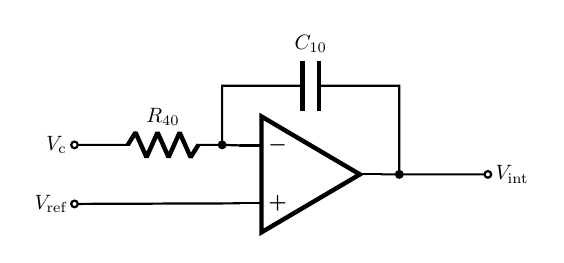
\begin{tikzpicture}[scale=0.75,transform shape]
    \draw[color=black, thick]
    (0,0) node [op amp] (int) {}
    (int.+) to[short,-o] (-4,-0.5) node [anchor=east] {$V_{\text{ref}}$}
    (int.-) to (-1.5,0.5) to[R,l_=$R_{40}$,*-] (-3.5,0.5) to[short,-o] (-4,0.5) node [anchor=east] {$V_{\text{c}}$}
    (-1.5,0.5) to (-1.5,1.5) to[C=$C_{10}$] (+1.5,1.5) to[short,-*] (+1.5,0) to (int.out)
    (+1.5,0) to [short,-o] (+3,0) node [anchor=west] {$V_{\text{int}}$}
    ;
  \end{tikzpicture}
\end{center}
The output voltage varies as
\begin{equation}
  \frac{dV_{\text{int}}}{dt} = -\frac{V_{\text{c}} - V_{\text{ref}}}{R_{40} C_{10}}
\end{equation}
With the values
\begin{center}
  \begin{tabular}{lS}
    \toprule
    $R_{40}$ & \SI{6.8}{\mega\ohm} \\
    $C_{10}$ & \SI{100}{\nano\farad} \\
    \bottomrule
  \end{tabular}
\end{center}
we get the time constant
\begin{equation}
  \tau = R_{40}C_{10} = \SI{0.68}{\second}
\end{equation}



\end{document}
